\documentclass[a4paper,11pt]{article}

\usepackage[french]{babel}
\usepackage[T1]{fontenc}
\usepackage[utf8]{inputenc}
\usepackage{graphicx}
%\usepackage{fullpage}

\begin{document}

\title{\textbf{Compte rendu du TP \no 4}\\Floutage du fond d'une image}
\author{Thibaut Castanié\\\textit{Master IMAGINA}}
\date{\today}

\maketitle
\thispagestyle{empty}

\newpage 

\section{Création d'une image couleur au format ppm}
L'image choisie pour la suite du TP est tirée du film Resident Evil: Afterlife. Le personnage au centre se détache de l'arrière-plan de façon nette. Le fond n'est pas trop éloigné et n'est donc pas déjà flouté par la profondeur de champ de la caméra.
\begin{center}
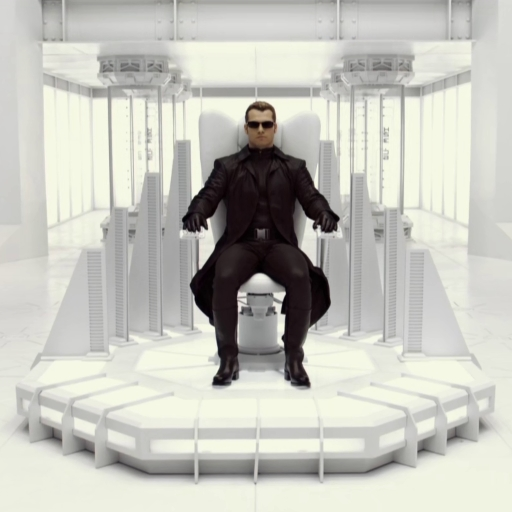
\includegraphics[scale=0.7]{wesker.png}\\
\textit{L'image originale couleur wesker.ppm}
\end{center}
\newpage
\section{Création d'une image en niveau de gris à partir d'une image couleur}
Pour obtenir une image en niveaux de gris, au format ppm, j'ai calculé la moyenne des niveaux de chaque couleur.
\begin{verbatim}
pour i de 0 à nbrePixelsImage
    pixelR = imageEntree[i*3];
    pixelG = imageEntree[(i*3)+1];
    pixelB = imageEntree[(i*3)+2];
    imageSortie[i] = moyenne(pixelR, pixelG, pixelB);
fin pour
\end{verbatim}
\vspace{1cm}
\begin{center}
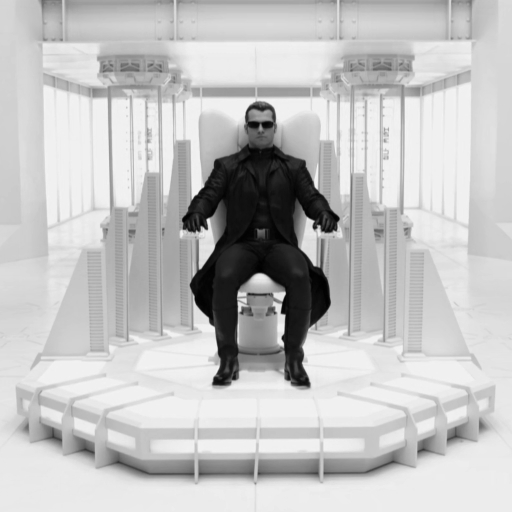
\includegraphics[scale=0.7]{weskergrisifie.png}\\
\textit{L'image wesker.pgm en niveaux de gris}
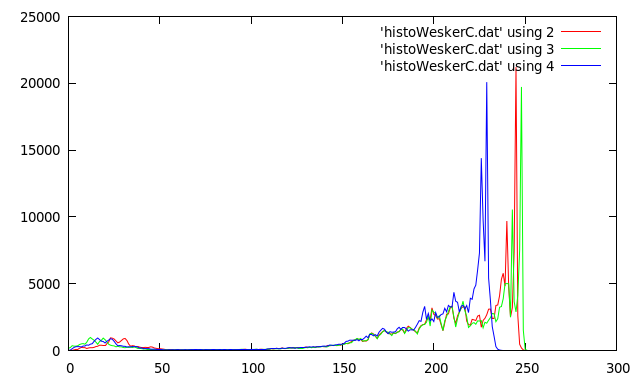
\includegraphics[scale=0.55]{histoWeskerC.png}
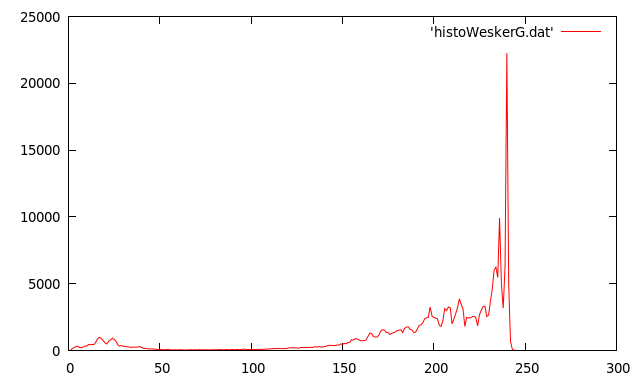
\includegraphics[scale=0.55]{histoWeskerG.png}\\
\textit{L'histogramme de wesker.ppm (couleur), et celui de wesker.pgm (gris)}
\end{center}

\newpage
\section{Seuillage de l'histogramme}
Sur l'image en niveau de gris, les pixels inférieurs à la valeur du seuil deviennent noirs, et ceux supérieurs deviennent blancs.

\begin{verbatim}
pour i de 0 à nbrePixelsImage
    si imageEntree[i] < seuilChoisi
        imageSortie[i] = 0;
    sinon
        imageSortie[i] = 255;
    fin si
fin pour
\end{verbatim}
\paragraph{} Après plusieurs tests effectués, nous utilisons une valeur de seuil de 180.
\begin{center}
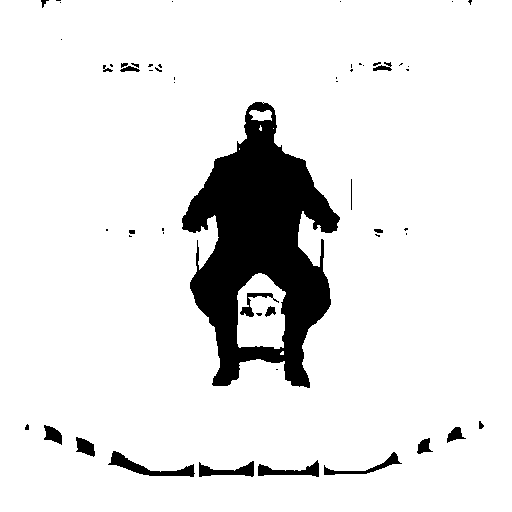
\includegraphics[scale=0.7]{weskerbinaire.png}\\
\textit{L'image weskerBinaire.pgm seuillée}
\end{center}

\newpage
\section{Floutage de l'image couleur}
\begin{verbatim}
pour i de 0 à nbrePixelsImage*3, i+=3
    imageSortie[i] = (imageEntree[i]+              //pixel central
                      imageEntree[i+3]+            //pixel de droite
                      imageEntree[i-3]+            //pixel de gauche
                      imageEntree[i+(nW*3)]+       //pixel du dessous
                      imageEntree[i-(nW*3)]+       //pixel du dessus
                      imageEntree[i+(nW*3)-3]+     //pixel bas-gauche
                      imageEntree[i+(nW*3)+3]+     //pixel bas-droit
                      imageEntree[i-(nW*3)+3]+     //pixel haut-droit
                      imageEntree[i-(nW*3)-3])     //pixel haut gauche
                      /9;
    imageSortie[i+1] = (imageEntree[i+1]+          //pixel central
                        imageEntree[i+4]+          //pixel de droite
                        imageEntree[i-2]+          //pixel de gauche
                        imageEntree[i+(nW*3)+1]+   //pixel du dessous
                        imageEntree[i-(nW*3)+1]+   //pixel du dessus
                        imageEntree[i+(nW*3)-2]+   //pixel bas-gauche
                        imageEntree[i+(nW*3)+4]+   //pixel bas-droit
                        imageEntree[i-(nW*3)+4]+   //pixel haut-droit
                        imageEntree[i-(nW*3)-2])   //pixel haut gauche
                        /9;
    imageSortie[i+2] = (imageEntree[i+2]+          //pixel central
                        imageEntree[i+5]+          //pixel de droite
                        imageEntree[i-1]+          //pixel de gauche
                        imageEntree[i+(nW*3)+2]+   //pixel du dessous
                        imageEntree[i-(nW*3)+2]+   //pixel du dessus
                        imageEntree[i+(nW*3)-1]+   //pixel bas-gauche
                        imageEntree[i+(nW*3)+5]+   //pixel bas-droit
                        imageEntree[i-(nW*3)+5]+   //pixel haut-droit
                        imageEntree[i-(nW*3)-1])   //pixel haut gauche
                        /9;
fin pour
\end{verbatim}
\begin{center}
\includegraphics[scale=0.7]{weskerFlou.png}\\
\textit{L'image floutée entièrement weskerFlou.ppm}
\end{center}

\newpage
\section{Floutage du fond de l'image couleur}
\begin{verbatim}
pour i de 0 à nbrePixelsImage*3, i+=3
    si imageBinaire[i/3] == 255
        imageSortie[i] = (imageEntree[i]+
                          imageEntree[i+3]+
                          imageEntree[i-3]+
                          imageEntree[i+(nW*3)]+
                          imageEntree[i-(nW*3)]+
                          imageEntree[i+(nW*3)-3]+
                          imageEntree[i+(nW*3)+3]+
                          imageEntree[i-(nW*3)+3]+
                          imageEntree[i-(nW*3)-3])
                          /9;
        imageSortie[i+1] = (imageEntree[i+1]+
                            imageEntree[i+4]+
                            imageEntree[i-2]+
                            imageEntree[i+(nW*3)+1]+
                            imageEntree[i-(nW*3)+1]+
                            imageEntree[i+(nW*3)-2]+
                            imageEntree[i+(nW*3)+4]+
                            imageEntree[i-(nW*3)+4]+
                            imageEntree[i-(nW*3)-2])
                            /9;
        imageSortie[i+2] = (imageEntree[i+2]+
                            imageEntree[i+5]+
                            imageEntree[i-1]+
                            imageEntree[i+(nW*3)+2]+
                            imageEntree[i-(nW*3)+2]+
                            imageEntree[i+(nW*3)-1]+ 
                            imageEntree[i+(nW*3)+5]+ 
                            imageEntree[i-(nW*3)+5]+
                            imageEntree[i-(nW*3)-1])
                            /9;
    sinon
        imageSortie[i] = imageEntree[i];
        imageSortie[i+1] = imageEntree[i+1];
        imageSortie[i+2] = imageEntree[i+2];
    fin si
fin pour
\end{verbatim}
\begin{center}
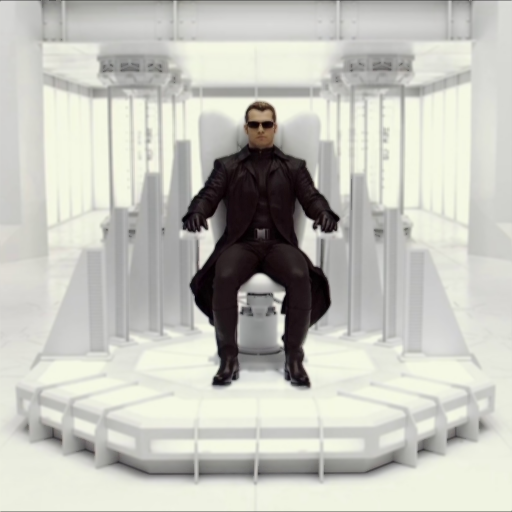
\includegraphics[scale=0.7]{weskerfondflou.png}\\
\textit{L'image avec seulement l'arrière plan flouté weskerFondFlou.ppm}
\end{center}

\newpage
\section{Érosion et dilatation}
Dans l'image obtenue précédemment, on remarque que quelques détails de l'arrière plan plus foncés n'ont pas étés floutés, car ils ressortent en noir sur l'image binaire. Pour arranger cela, trois érosions, suivies de 3 dilatations ont étés effectuées.
\begin{verbatim}
//erosion
pour i de 0 à nbrePixelsImage
    si imageEntree[i] == 255
        imageSortie[i] = 255        //pixel central
        imageSortie[i+1] = 255      //pixel de droite
        imageSortie[i+2] = 255      //pixel de gauche
        imageSortie[i-nW] = 255     //pixel du dessus
        imageSortie[i+nW] = 255     //pixel du dessous
    fin si
fin pour

//dilatation
pour i de 0 à nbrePixelsImage
    si imageEntree[i] == 0
        imageSortie[i] = 0        //pixel central
        imageSortie[i+1] = 0      //pixel de droite
        imageSortie[i+2] = 0      //pixel de gauche
        imageSortie[i-nW] = 0     //pixel du dessus
        imageSortie[i+nW] = 0     //pixel du dessous
    sinon
        imageSortie[i] = 255
    fin si
fin pour
\end{verbatim}
\begin{center}
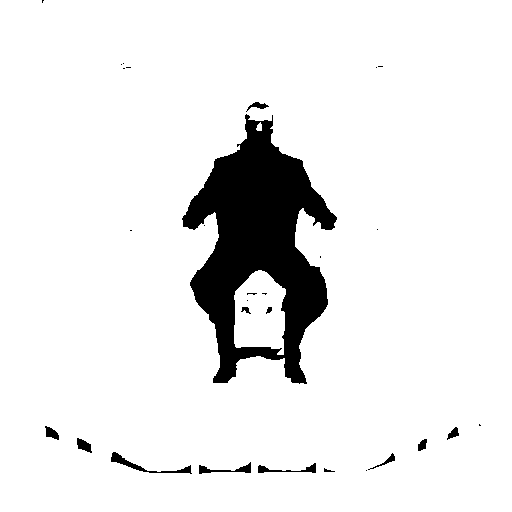
\includegraphics[scale=0.33]{weskerbinaireeee.png}
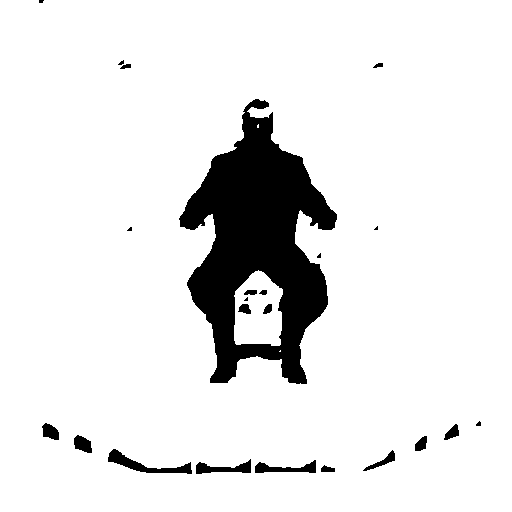
\includegraphics[scale=0.33]{weskerbinaireeeeddd.png}\\
\textit{L'image binaire ayant subit 3 érosion, puis 3 dilatations}
\end{center}

\paragraph{} En appliquant de nouveau l'algorithme de la question 5 en utilisant notre nouvelle image binaire, on obtient l'image suivante.
\begin{center}
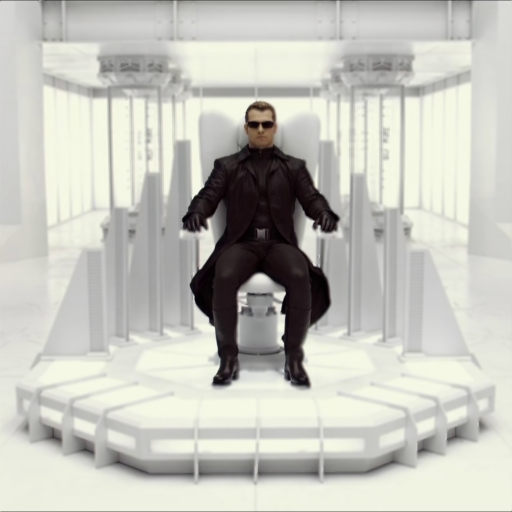
\includegraphics[scale=0.7]{weskerfondfloumieux.png}\\
\textit{L'image avec l'arrière plan flouté amélioré}
\end{center}


\end{document}